\section{Approach}
\subsection{Preliminaries}
\noindent \textbf{Segment Anything.} SAM~\citep{kirillov2023segment} contains a  ViT image encoder and a prompt-guided mask decoder. The encoder takes an image and outputs image embeddings. Then the decoder takes the image embeddings and a prompt, which allows cutting out any object from the background in an image. 
SAM is trained on an image dataset of over 1B masks.
% SAM is trained on SA-1B, an image dataset of over 1B masks from 11M images~\citep{kirillov2023segment}.

\noindent \textbf{Segment Anything 2.} The architecture of segment anything 2 (SAM 2)~\citep{ravi2024sam} largely follows SAM, which consists of a hierarchical image encoder, a prompt-guided lightweight mask decoder, and a new memory mechanism. SAM 2 uses a hierarchical image encoder, Hiera~\citep{ryali2023hiera}, to produce image embeddings for each frame. The stride 16 and 32 features from Stage 3 and 4 are used for the memory module. The stride 4 and 8 features from Stage 1 and Stage 2 are not used in the memory module but are fed to upsampling layers in the mask decoder for generating segmentation masks. For stable object tracking, SAM 2 employs a memory mechanism consisting of a lightweight memory encoder, a lightweight memory bank, and a memory attention module. It stores information from past frames and uses the memory attention module to perform cross-attention between the stored memory in the memory bank and current frame features, thereby understanding temporal dependencies in video.

The memory attention module consists of a stack of transformer blocks. Each block contains self-attention, cross-attention, and MLP. The first transformer block takes the image embedding from the current frame as an input. The core component of each transformer block, cross-attention, integrates the current frame embedding and the memory stored in memory bank to produce an embedding with temporal correspondence information. 
% Let us denote the memory bank as,
% \begin{equation*} 
%     \begin{split}
%     M_{b} = [m_{11}; \dots; m_{1N}; \dots, m_{T1}; \dots; m_{TN}] \in \R^{TN \times d_m},
%     \end{split}
% \end{equation*}
% where $T$ is the number of frames saved in the memory, $N$ is the number of memory tokens per frame, $d_m$ is the channel dimension. 
For memory tokens, it includes two parts, the spatial embedding tokens from memory encoder and the object-level pointer tokens from mask decoder. 
% Let us assume the resolution of spatial embedding tokens is $w \times h$, 
Let us assume the number of spatial tokens is $n$, the number of object-level pointer tokens is $P$, and $d_m$ is the channel dimension, memory tokens can be formulated as $
M_{b} = \begin{bmatrix} 
    M_s\in \R^{n\times d_m}\\
    M_p\in \R^{P\times d_m}
    \end{bmatrix}.
$
% \begin{equation} \label{equ:mbank}
%     \begin{split}
%     M_{b} = & [m_{11}; \dots; m_{1wh}; \dots, m_{1wh+P}; \\
%     & \vdots \dots \dots \vdots \dots \dots \vdots \dots \dots \vdots,\\
%     & m_{T1}; \dots; m_{Twh}; \dots, m_{T(wh+P)}]
%     \end{split}
% \end{equation}
% \[
% M_{b} = \begin{bmatrix} 
%     m_{11}; & \dots  & m_{1wh}; & \dots & m_{1wh};\\
%     \vdots & \dots & \vdots & \dots & \vdots\\
%     m_{T1}; & \dots  & m_{Twh}; &\dots & m_{Twh+P};
%     \end{bmatrix}
% \]

Let $L$ be the number of tokens and $d_q$ be the dimension of each token for input frame features after self-attention, $X \in \R^{L \times d_q}$. The input sequence $X \in \R^{L \times d_q}$ is linearly projected to input queries $Q \in \R^{L\times d}$, and the memory tokens, $M_{b} \in \R^{(n+P)\times d_m}$ are linearly projected to keys $K \in \R^{(n+P) \times d}$, and values $V \in \R^{(n+P) \times d}$ respectively, where $d$ is the embedding dimension of queries, keys, and values. The scaled dot-product cross attention mechanism applied on the queries $Q$, keys $K$, values $V$ can be formally written as, 
\begin{equation}\label{eq:crossattn}
     \textsf{C}(Q, K, V) =  \text{softmax}\Lleft\frac{QK^T}{\sqrt{d}}\Rright V,
\end{equation}
where the $\text{softmax}$ operation is applied row-wise. A single head cross attention is used in the memory module. In later discussion, we also consider keys and values as memory tokens for simplification. 
% The scaling $\sqrt{d}$ will be omitted in later discussion to simplify notation.

\noindent \textbf{Efficiency Bottleneck.} Despite the advantages of the hierarchical image encoder for multiscale frame feature extraction and cross-attention for integrating current frame features with stored memory, it poses the challenges for practical deployment of SAM 2. The inefficient SAM 2 (tiny) even shows comparable FPS to the base SAM 2, 47.2 FPS vs 43.8 FPS due to the hierarchical design of the image encoder and the use of hierarchical features, which also makes SAM 2 challenging to deploy on mobile devices. Moreover, the number of tokens in keys and values for performing cross-attention in the memory module are super long, e.g., $30K$. It leads to a large computation and memory cost when performing cross-attention, which becomes the efficiency bottleneck of the memory module for real-world deployment. 

\begin{figure*}[t]
    \centering
    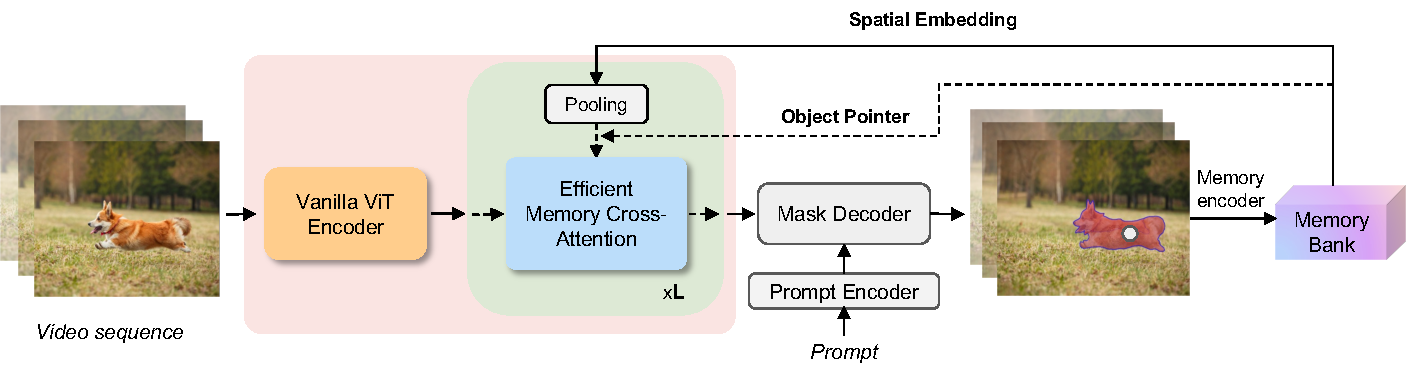
\includegraphics[width=0.9\textwidth]{figures/arch.pdf}
    \caption{EfficientTAM architecture. Our proposed EfficientTAM takes a vanilla lightweight ViT image encoder for frame feature extraction. An efficient memory cross-attention is proposed to further improve the efficiency of EfficientTAM by leveraging the strong locality of memory spatial embeddings. EfficientTAM is fully trained on SA-1B (image) and SA-V (video) for unified image and video segmentation.}
    \label{fig:efficienttams}
\end{figure*}

\subsection{Efficient Video Object Segmentation and Track Anything} 
We now address the efficiency issue of SAM 2 for building efficient video object segmentation and track anything model, EfficientTAM. Motivated by the high quality segmentation performance of SAM and EfficientSAM, we revisit using plain, non-hierarchical lightweight image encoders such as ViT-Small/ViT-Tiny, for frame feature extraction. We found that the use of vanilla ViT for frame feature extraction makes EfficientTAM highly efficient and deployable on mobile devices. Further, we introduce an efficient memory module to reduce the computation and memory cost by proposing an efficient cross-attention operation. Based on these two designs, we build efficient video object segmentation and track anything model by largely following SAM2.  \cref{fig:efficienttams} illusrates an overview of our proposed EfficientTAM. 

\noindent \textbf{Efficient Image Encoder.} The image encoder's role is to produce feature embeddings for each high-resolution frame. We use a SAMI~\citep{xiong2024efficientsam} pretrained vanilla ViT image encoder~\citep{dosovitskiy2020image,touvron2021training} to extract frame features. Differing from the image encoder of SAM 2, our image encoder provides a single-scale feature map and no other features in the mask decoder are added to the upsampling layers during decoding for segmentation mask generation. We adopt the lightweight image encoders ViT-Small and ViT-Tiny with a $16\times 16$ patch size. Following \citep{li2022exploring}, we use $14\times 14$ non-overlapping windowed attention and 4 equally-spaced global attention blocks to efficiently extract features from high-resolution frames. Our image encoder outputs a single-scale feature embedding with a $16$x reduced resolution, which takes high-resolution (e.g., $1024\times 1024$) frames as input and transforms it into a dense embedding of downscaled size $64\times 64$. 

\begin{figure*}[t]
    \centering
    \begin{overpic}[width=1.0\linewidth]{figures/cross_attention.png}
\put (7,19) {\scriptsize{Keys}}
\put (22,19) {\scriptsize{Coarse Keys}}
\put (45,19) {\scriptsize{Values}}
\put (61,19) {\scriptsize{Coarse Values}}
\put (79,19) {\scriptsize{Absolute Cross-Attention Error }}
\end{overpic}
    \caption{An example to show strong locality of the Keys and Values in the cross-attention of the memory module. Keys and Values are a matrix of size $28700\times 256$. Cross-attention is a matrix of size $4096\times 256$. For simplicity of visualizing and comparison, we only draw the top matrix of size $320\times256$. We use a single averaged token to represent other tokens in the homogeneous window with a $2\times 2$ size, for Keys and Values to obtain coarse Keys and Values. At right, we visualize the difference between original cross-attention of \cref{eq:crossattn} and efficient cross-attention of \cref{eq:ecrossattn}; the relative error w.r.t original cross-attention is $0.03$ under Frobenius norm.}
    \label{fig:cross_attn}
% \vspace{-3mm}
\end{figure*}

% The difference between original cross-attention of \cref{eq:crossattn} and efficient cross-attention of \cref{eq:ecrossattn} with coarse Keys and Values is marginal, visualized at the right. The relative error w.r.t. original cross-attention is $0.03$ under Frobenius norm. 

\noindent \textbf{Efficient Memory Module.} The memory module leverages information from previous frames to facilitate consistent object tracking. Cross-attention is a major efficiency bottleneck of the memory module in SAM 2~\citep{ravi2024sam} due to its long memory token sequence. We now discuss how exploiting the underlying structure of memory tokens --- local smoothness (strong locality) within spatial memory tokens --- can yield a more efficient cross-attention. 

Consider two consecutive memory spatial tokens, $k_i$ and $k_{i+1}$, local smoothness  implies that $||k_i - k_{i+1}||^2_2 \leq \frac{c_K}{n^2}$, for $i = 1, \dots, n - 1$, where $c_K$ is a positive constant. 
This suggests that given a sufficient small local window, $l_w \times l_h$, using a single token to represent other tokens in the homogeneous window may provide a coarser representation of the full set of memory spatial tokens $K_s$ as $\Tilde{K}_s$. We can construct a good surrogate of $K_s$ with the same size, $\Bar{K}_s$, from $\Tilde{K}_s$ by repeating the single token in each window $l_w\times l_h$ times. Under the smoothness assumption, $\Bar{K}_s$ will not be far from $K_s$. Empirically, we observed that a coarser representation of spatial memory tokens is good surrogate of the full spatial memory tokens. \cref{fig:cross_attn} confirms the coarser representation of input keys and values are close to the original keys and values of cross-attention in the memory module. 

Utilizing highly correlated neighboring tokens in cross-attention, we perform average pooling to efficiently compute a coarser representation for keys $K$ and values $V$ in our model. For input spatial tokens $K_s = [k_{11}, \dots, k_{1h}; \dots; k_{w1}, \dots, k_{wh}]$ where $w \times h$ is the resolution size, we divide the $n = w\times h$ tokens into $k = \Tilde{w}\times \Tilde{h}$ rectangular pooling regions and compute the average token of each region. For simplicity, we assume $w$ is divisible by $\Tilde{w}$ and $h$ is divisible by $\Tilde{h}$. Denote $l_w = \frac{w}{\Tilde{w}}, l_h = \frac{h}{\Tilde{h}}$. $\Tilde{K}_s$ and $\Tilde{V}_s$ can be computed by averaging each region as,   
\begin{align}\label{eq:keys-values}
\small
\Tilde{k}_{ij} & = \sum_{p = i \times l_w + 1}^{(i + 1) \times l_w}\sum_{q = j \times l_h + 1}^{(j + 1) \times l_h} \frac{k_{pq}}{l_w \times l_h}, \nonumber \\
\Tilde{v}_{ij} & = \sum_{p = i \times l_w + 1}^{(i + 1) \times l_w}\sum_{q = j \times l_h + 1}^{(j + 1) \times l_h} \frac{v_{pq}}{l_w \times l_h}, 
\end{align}
where $i = 1, \cdots, \Tilde{w}, j=1, \cdots, \Tilde{h}$. This token-pooling scheme requires a single scan
of the tokens leading to an efficient coarse token generation. We find that using averaging pooling with window size, $2 \times 2$, is sufficient to ensure a good approximation for spatial memory tokens. 

Assume $\Tilde{K}_s$ is a coarser representation of memory spatial keys, $K_s$, we can construct a good surrogate of $K_s \in \R^{n \times d}$ with the same size, $\Bar{K}_s \in \R^{n \times d}$ from $\Tilde{K}_s \in \R^{\Tilde{w}\Tilde{h} \times d}$ by stacking each $\Tilde{k}_i, i = 1, \dots, \Tilde{w}\Tilde{h}$, $l_w\times l_h$ times, which can be written as,
\begin{align*}
    \Bar{K}_s = [\underbrace{\Tilde{k}_1; \dots; \Tilde{k}_1}_{l_w\times l_h}; \underbrace{\Tilde{k}_2; \dots; \Tilde{k}_2}_{l_w\times l_h}; \dots; \underbrace{\Tilde{k}_{\Tilde{w}\Tilde{h}}; \dots; \Tilde{k}_{\Tilde{w}\Tilde{h}}}_{l_w\times l_h}]
\end{align*}
Similarly, we stack each $\Tilde{v}_i, i =1, \dots, \Tilde{w}\Tilde{h}$, $l_w\times l_h$ times to construct $\Bar{V}_s  \in \R^{n \times d}$ as a good surrogate of values, $V_s \in \R^{n\times d}$, which can be written as,
\begin{align*}
    \small 
    \Bar{V}_s= [\underbrace{\Tilde{v}_1; \dots; \Tilde{v}_1}_{l_w\times l_h}; \underbrace{\Tilde{v}_2; \dots; \Tilde{v}_2}_{l_w \times l_h}; \dots; \underbrace{\Tilde{v}_{\Tilde{w}\Tilde{h}}; \dots; \Tilde{v}_{\Tilde{w}\Tilde{h}}}_{l_w \times l_h}]
\end{align*}
% With the stacked $\Bar{K}_s \in \R^{n \times d}$, $\Bar{V}_s \in \R^{n \times d}$,
Then we concatenate this coarse spatial tokens with object pointer tokens, $\Bar{K} = [\Bar{K}_s; K_p]\in \R^{(n+P)\times d}$ and $\Bar{V} = [\Bar{V}_s; K_p]\in \R^{(n+P)\times d}$, for a good surrogate of original memory tokens, $K$ and $V$. For the coarse memory tokens, $\bar{K}$ and $\bar{V}$, we have,
% \begin{align}\label{eq:replace}
%     \text{softmax}\Lleft\frac{Q\Bar{K}^{T}}{\sqrt{d}}\Rright\Bar{V} = \text{softmax}\Lleft\frac{Q\Tilde{K}^{T}}{\sqrt{d}} + \ln{(l_w\times l_h)}\Rright\Tilde{V},
% \end{align}
\begin{align}\label{eq:replace}
    \text{softmax}\Lleft\frac{Q\Bar{K}^{T}}{\sqrt{d}}\Rright\Bar{V} = \text{softmax}\Lleft A \Rright\Tilde{V},
\end{align}
where $A = [\frac{Q\Tilde{K}_s^{T}}{\sqrt{d}} + \ln{(l_w\times l_h)}, \frac{QK_p^{T}}{\sqrt{d}}] \in \R^{L\times (\Tilde{w}\Tilde{h} + P)}$, $\Tilde{V} = [\Tilde{V}_s; V_p] \in \R^{(\Tilde{w}\Tilde{h}+P)\times d}$. We provide a proof of \cref{eq:replace} in the appendix. 
Since $\Bar{K}$ and $\Bar{V}$ are good surrogate of $K$ and $V$ respectively, we obtain a good surrogate of the original cross-attention, $\text{softmax}\Lleft\frac{QK^T}{\sqrt{d}}\Rright V$ in \cref{eq:crossattn},
\begin{equation}\label{eq:scrossattn}
     \Bar{\textsf{C}}(Q, K, V) =  \text{softmax}\Lleft\frac{Q\bar{K}^T}{\sqrt{d}}\Rright \bar{V}.
\end{equation}
With \cref{eq:replace}, we have an efficient version of cross-attention, 
\begin{equation}\label{eq:ecrossattn}
     \Bar{\textsf{C}}(Q, K, V) = \text{softmax}(A)\Tilde{V}.
\end{equation}
% \begin{equation}\label{eq:ecrossattn}
%      \Bar{\textsf{C}}(Q, K, V) = \text{softmax}\Lleft\frac{Q\Tilde{K}^{T}}{\sqrt{d}} + \ln{(l_w\times l_h)}\Rright\Tilde{V},
% \end{equation}
\noindent\textbf{Link to efficient cross-attention variants.} Interestingly, we can find some cross-attention variants based on our proposed efficient cross-attention in  \cref{eq:ecrossattn}. We notice there is a constant for balancing the attention score between coarse spatial tokens and object pointer tokens, avoiding reducing the attention to spatial tokens after pooling. If we remove this constant, it can lead to a linformer variant using averaging pooling to replace the learnable projection. Instead of removing the constant, we add it to keys for regularizing the attention between coarse spatial tokens and object pointer tokens in \cref{eq:acrossattn}, for obtaining another variant. 

\begin{equation}\label{eq:acrossattn}
     \Tilde{\textsf{C}}(Q, K, V) = \text{softmax}\Lleft\frac{Q\Tilde{K}^{T}}{\sqrt{d}} \Rright\Tilde{V},
\end{equation}
where $\Tilde{K} = [\Tilde{K}_s + \ln{(l_w\times l_h)}, K_p]\in\R^{(\Tilde{w}\Tilde{h}+P)\times d}$.

It is feasible to achieve a good surrogate of the original cross-attention because spatial memory embeddings have strong locality. 
% since the neighboring tokens are similar. 
Our efficient cross-attention is close to the original cross-attention, visualized in \cref{fig:cross_attn}. 
% We can also obtain a upper error bound of the efficient version of cross-attention in \cref{eq:ecrossattn} w.r.t the original cross-attention in \cref{eq:crossattn} under the smooth assumption, included in the supplement.
% Since our efficient cross attention method exploits locality of memory tokens, it becomes more suitable with some guarantees of its behavior.
% Detailed proof is included in the supplement. 
% Assume keys $K = [k_1; \dots; k_n] \in \mathbf{R}^{n \times d_k}$ and values $V =[v_1; \dots; v_n] \in \mathbf{R}^{n \times d}$ are smooth, i.e., $||k_i - k_{i+1}||^2_2 \leq \frac{c_K}{n^2}$, and $||v_i - v_{i+1}||^2_2 \leq \frac{c_V}{n^2}$, $i = 1, \dots, n - 1$, $c_K, c_V$ are positive constants. Let us denote $\Tilde{K} = [\Tilde{k}_1; \dots; \Tilde{k}_k]$, where $\Tilde{k}_i \in \R^{1 \times d}$, and $\Tilde{V} = [\Tilde{v}_1; \dots; \Tilde{v}_k]$, where $\Tilde{v}_i \in \R^{1 \times d}$ from keys $K$ and $V$ by applying token-pooling. We have the following upper bound for the error $||\textsf{C}(Q, K, V) - \Bar{\textsf{C}}(Q, K, V)||_{\text{Fro}}$,
% \begin{lemma}\label{lem:upperbound}
% Assume keys $K \in \mathbf{R}^{n \times d}$ and values $V \in \mathbf{R}^{n \times d}$ are smooth. For queries $Q \in \mathbf{R}^{n \times d}$, cross-attention matrix $\Bar{\textsf{C}}(Q, K, V)$, $\Tilde{K} \in \mathbf{R}^{k \times d}$, $\bar{V} \in \mathbf{R}^{n \times d}$, we have for $k \geq \frac{\max{(c_K, c_V)}}{\epsilon^2}$
% \begin{equation}\label{eq:bnd}
%      ||\Bar{\textsf{C}}(Q, K, V) - \textsf{C}(Q, K, V)||_{\text{Fro}} \leq \epsilon (\frac{||Q||_2}{\sqrt{d_k}}||V||_2 + 1)
% \end{equation}
% \end{lemma}
% Lemma \ref{lem:upperbound} suggests that our efficient cross-attention is close to the original cross-attention when window size of averaging pooling is small. We note that it is feasible to achieve a good  surrogate of the original cross-attention. This is because spatial memory embeddings have strong locality since the neighboring tokens are similar. Since our efficient cross attention method exploits locality of memory tokens, it becomes more suitable with some guarantees of its behavior.









